\chapter{ТЕОРЕТИЧЕСКАЯ ЧАСТЬ}

\section{Развитие генераторов сигналов}
	История развития генераторов сигналов начинается с аналоговых устройств, которые
использовались для генерации различных форм сигналов, включая низкочастотные,
высокочастотные, сверхвысокочастотные и импульсные. Во времена СССР разрабатывалось большое количество аналоговых генераторов сигналов \cite{dgs}. Однако, с развитием технологий и потребностями в более сложных и модулируемых сигналах, стала очевидна необходимость в усовершенствовании источников сигнала.

	В результате развития технологий появились цифровые генераторы на основе прямого цифрового синтеза частот и форм сигналов. Цифровые генераторы сигналов используют минимальное количество аналоговой элементной базы и основываются на специализированных сверхскоростных цифровых микросхемах, а также аналого-цифровых (АЦП) и цифро-аналоговых (ЦАП) преобразователях. Благодаря этому, интеграция данных генераторов с цифровыми системами становится легкой и позволяет открыть массу перспектив их использования в процессе тестирования и наладки разнообразных электронных и радиотехнических устройств. 

	В современной измерительной технике генераторы сигналов играют ключевую роль во многих сферах. %Несмотря на то, что в прошлом развитие в этой области было активно, в настоящее время наблюдается отставание от многих передовых направлений применения электронных устройств, включая микропроцессоры, работающие на частотах в единицы ГГц и выше. 
	В целом, история развития генераторов сигналов отражает эволюцию технологий, потребностей в модулируемых сигналах и влияние глобальных изменений в науке и технике.

\section{Основные типы сигналов}
	Для начала стоит дать определение, что такое сигнал. Сигнал --- это носитель информации. Он является переносчиком знаков, которые вместе образуют основу информации для передачи сообщения. Исходя из этого можно сделать вывод, что постоянные токи и напряжения сигналами не являются, т.к. их параметры во времени не меняются, но впрочем их можно отнести к простейшим сигналам, которые несут в себе информацию о полярности величины. В качестве сигналов они конечно не используются, но с помощью них можно задавать смещение сигналам~\cite{dgs}.

	Рассмотрим некоторые распространённые типы сигналов.
\subsection{Синусоидальные сигналы}
	Именно синусоидальные сигналы мы извлекаем из розетки. Математическое выражение, описывающее синусоидальное напряжение, имеет вид:
	\begin{gather}
	U=A sin2 \pi ft,
	\end{gather}
	где А --- амплитуда сигнала,
	
	$f$ --- частота в герцах.

	\begin{figure}[H]
    \centering
    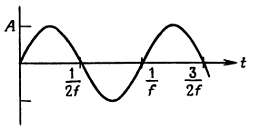
\includegraphics[width=0.575\textwidth]{../image/s_sin.png}
    \caption{Синусоидальный сигнал.}
	\end{figure}
	Эффективное значение равняется двойной амплитуде, то есть размаху сигнала. 

	Если нужно переместить начало координат ($t=0$) в какой-то момент времени, то в формулу следует добавить фазу:
	\begin{gather}
	U=A sin2 \pi ft + \theta,
	\end{gather}
	
	Синусоидальные сигналы характеризуются тремя параметрами:
	\begin{itemize}
		\item $U_{M}$ или $I_{M}$ --- амплитуда переменного напряжения или тока;
		\item $f$ --- частота (период);
		\item $\theta$ --- фазовый сдвиг.
	\end{itemize}

	Данный тип сигналов является периодическим, т. е. временная зависимость повторяется и есть условия:
	\begin{gather}
	u(t)=u(t+T),\\
	i(t)=i(t+T), 
	\end{gather}
	
	где $T=\dfrac{1}{f}$ --- период повторения сигнала.
	
	У синусоиды есть своё достоинство в том, что функция данной формы сигнала является решением многих дифференциальных уравнений, которые описывают как физические явления, так и свойства линейных цепей ~\cite{is1}. На практике поведение схемы оценивают по её амплитудно-частотной характеристике (АЧХ), которая показывает, как изменяется амплитуда синусоидального сигнала в зависимости от частоты. Для примера на усилителе звуковых частот амплитудно-частотная характеристика в идеале имеет ровную линию в диапазоне от 20 Гц до 20 кГц. Чаще всего частоты, с которыми приходится работать на синусоидальном сигнале, лежат в диапазоне от нескольких герц до нескольких мегагерц.

\subsection{Линейно-меняющийся сигнал}
	Линейно-меняющийся сигнал --- это напряжение, возрастающее (или убывающее) с постоянной скоростью.

\begin{figure}[H]
     \begin{subfigure}[H]{0.45\textwidth}
         \centering
         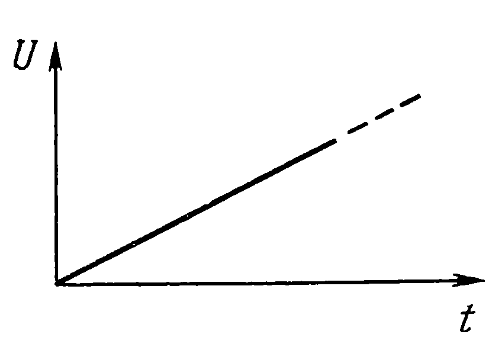
\includegraphics[width=0.70\textwidth]{../image/s_la.png}
         \caption{Возрастающее напряжение в виде сигнала.}
     \end{subfigure}
     \hfill
     \begin{subfigure}[H]{0.45\textwidth}
         \centering
         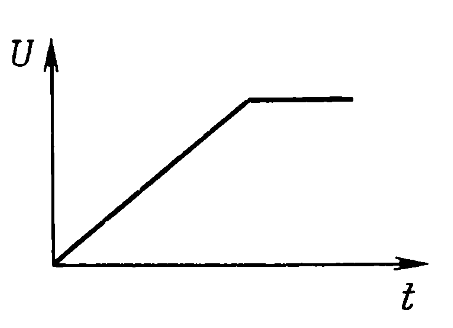
\includegraphics[width=0.70\textwidth]{../image/s_lb.png}
         \caption{Ограниченный сигнал.}
     \end{subfigure}
        \caption{Линейно-меняющийся сигнал.}
\end{figure}

	Напряжение не может, конечно, расти бесконечно. Поэтому обычно данная величина имеет конечное значение (рис. 1.2 (б)) или сигнал становиться пилообразным (рис. 1.3).

	\begin{figure}[H]
    \centering
    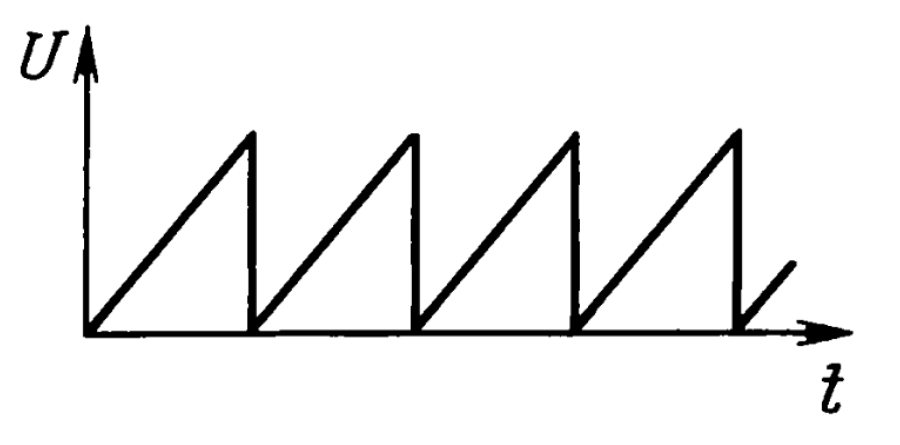
\includegraphics[width=0.45\textwidth]{../image/s_saw.png}
    \caption{Пилообразный сигнал.}
	\end{figure}

\subsection{Треугольный сигнал}
	Треугольный сигнал очень похож на линейно-меняющийся, но его отличие в том, что он симметричный.

	\begin{figure}[H]
    \centering
    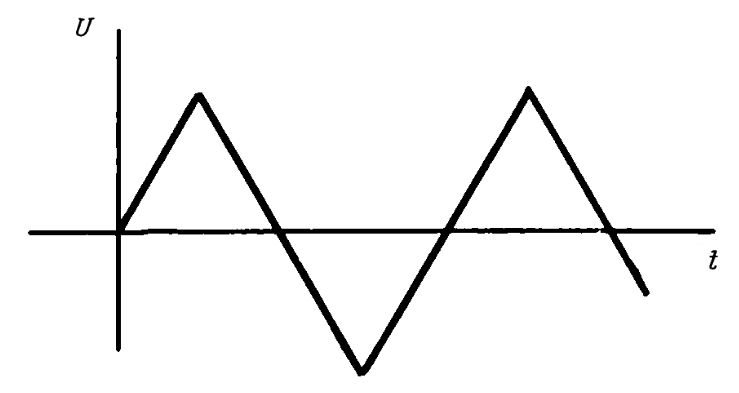
\includegraphics[width=0.35\textwidth]{../image/s_tri.png}
    \caption{Треугольный сигнал.}
	\end{figure}

\subsection{Шум}
	
	Также существует потребность в генерации шумов для анализа реакции на такой сигнал схемы. Характеризуется частотным спектром (произведение мощности на частоту в герцах)~\cite{is1}. Самое распространённое шумовое напряжение --- белый шум с распределением Гаусса.  

	\begin{figure}[H]
    \centering
    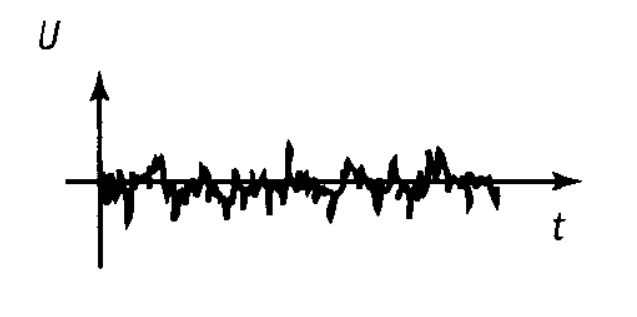
\includegraphics[width=0.45\textwidth]{../image/s_noise.png}
    \caption{Сигнал шума.}
	\end{figure}

\subsection{Прямоугольный сигнал}
	Прямоугольный сигнал или как его ещё называют меандр, характеризуется так же как и синусоидальный сигнал частотой и амплитудой.
	\begin{figure}[H]
    \centering
    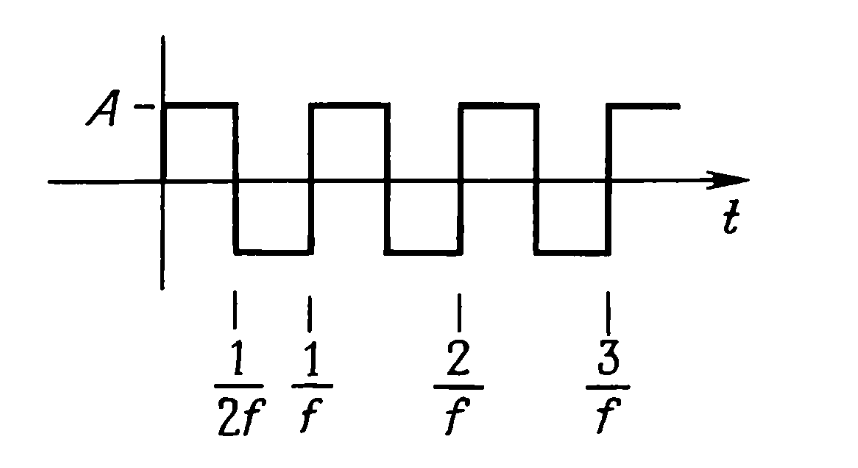
\includegraphics[width=0.45\textwidth]{../image/s_p.png}
    \caption{Прямоугольный сигнал.}
	\end{figure}

	Эффективным значением для данного сигнала является значение его амплитуды. На самом деле прямоугольный сигнал не идеален. Его форма отличается от прямоугольника, т.к. присутствует время нарастания $t_{H}$, которое может быть от нескольких наносекунд до нескольких микросекунд~\cite{is1}.

	\begin{figure}[H]
    \centering
    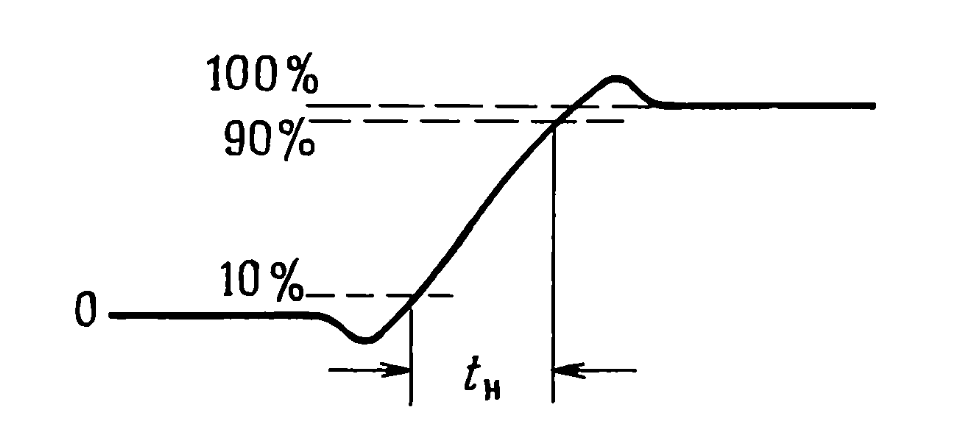
\includegraphics[width=0.7\textwidth]{../image/s_p_t.png}
    \caption{Время нарастания скачка прямоугольного сигнала.}
	\end{figure}
	
	На рисунке 1.7 изображено как обычно выглядит скачок сигнала прямоугольника. Время когда сигнал нарастет определяется в промежутке от 10 до 90\% максимальной амплитуды сигнала.

\subsection{Импульсы}
Сигналы в виде импульса изображены на рисунке 1.8.

	\begin{figure}[H]
    \centering
    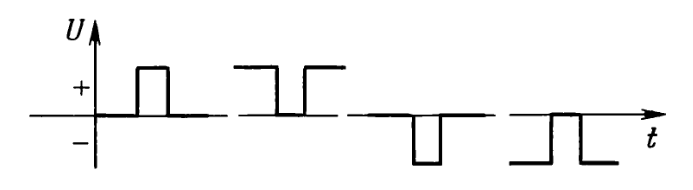
\includegraphics[width=0.65\textwidth]{../image/s_i.png}
    \caption{Импульсы.}
	\end{figure}
	
	Данный вид сигналов характеризуется амплитудой и длительностью импульса. Можно генерировать последовательность периодических импульсов и тогда можно ещё характеризовать сигнал частотой (повторением импульса). У импульсов есть полярность --- положительная и отрицательная. Кроме этого импульс может спадать, а может нарастать. 
	


\subsection{Скачки и пики}
	Часто можно слышать о сигналах в виде скачков и пиков, но на самом деле широкого применения они не находят. С помощью них обычно описывают работу схемы. Данный вид сигналов изображён на рисунке 1.9.

	\begin{figure}[H]
    \centering
    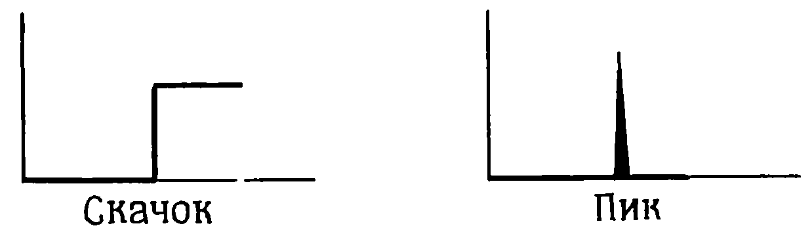
\includegraphics[width=0.6\textwidth]{../image/s_sp.png}
    \caption{Сигнал в виде скачка и пика.}
	\end{figure}

	Скачок представляет из себя отдельную часть прямоугольного сигнала, в то время как пик представляет собой два скачка, разделенных очень коротким промежутком.


\section{Виды генераторов}
	Источник сигнала часто является неотъемлемой частью схемы, но для тестирования работы удобно иметь отдельный, независимый источник сигнала. В качестве такого источника могут использоваться следующие виды генераторов.
\begin{enumerate}
	\item Генераторы синусоидальных сигналов.
	\item Функциональные генераторы.
	\item Генераторы сигналов произвольной формы.
	\item Генераторы импульсов.
\end{enumerate}

\subsection{Генераторы синусоидальных сигналов}
	Генераторы таких сигналов широко применяются при тестировании различных радиоэлектронных устройств. Сами же синусоидальные сигналы являются простейшими. Они изменяются во времени, но их параметры --- амплитуда, частота и фаза остаются постоянными~\cite{dgs}. Изменяя эти параметры, возможно осуществить модуляцию синусоидальных сигналов и использовать их для переноса информации. На таком принципе построены разнообразные области применения синусоидальных сигналов в радиотехнике.

	В области измерительных приборов существуют различные виды генераторов синусоидального напряжения. Одни из них схемы на RC-цепи для генерации низкочастотных сигналов и на основе LC-контуров для высокочастотных сигналов, далее конструировались схемы на основе разных типов резонаторов, но всё это уже прошлый век и на данный момент генераторы синусоидального сигнала строятся на основе цифровых методах синтеза.

%\begin{enumerate}
%	\item Высокочастотные LC-генераторы.
%	\item Низкочастотные RC-генераторы.
%	\item Генераторы с разными типами резонаторов (кварцевые, пьезоэлектрические).
%	\item Генераторы, которые формируют синусоиды, плавно ограничивая сигнал треугольника.
%	\item Генераторы построенные на основе цифровых методах синтеза синусоидального сигнала.
%\end{enumerate}

%	Конечно в настоящее время первые четыре типа генераторов уже прошлый век. Развитие цифровых и вычислительных технологий способствовало созданию и широкому распространению генераторов пятого типа, которые используют цифровые методы для генерации синусоидальных и различных других форм сигналов.

\subsection{Функциональные генераторы}
	Функциональными генераторами обычно называют генераторы, которые могут создавать несколько функциональных зависимостей. Данные устройства генерируют сигналы разной формы. Их простота и плавная регулировка частоты в большом диапазоне привела к массовому применению генераторов такого типа. Из всех генераторов, генераторы функций являются очень гибкими. Они позволяют генерировать синусоидальные, треугольные и прямоугольные сигналы в широком спектре частот, при этом возможно регулировать амплитуду и смещать сигнал по постоянному току. Благодаря такому разнообразию сигналов, сфера применения таких генераторов сильно расширяется. Данный вид источника сигнала может быть одним на все случаи жизни. Их можно использовать для тестирования, исследования и отладки абсолютно разной электронной аппаратуры.

	Функциональные генераторы также существуют как аналоговые так и цифровые, но в настоящее время аналоговые неактуальны. Переход к функциональным генераторам с цифровым синтезов выходных сигналов и цифровой элементной базой связан с растущими требованиями к сигналам источника~\cite{dgs}. У сигнала должна быть стабильная частота с амплитудой и верная форма. Благодаря применению цифровых элементов в массовой продукции (персональный компьютер, мобильный телефон), цифровые интегральные схемы стали бурно развиваться. Стала повышаться функциональность схем и понижаться их стоимость.

\subsection{Генераторы сигналов произвольной формы}
	Данный вид генератора дополняет функциональный генератор. Достаточно новое направление в генераторах сигналов, которое основывается на прямом цифровом синтезе различных сигналов, по сути произвольных форм. Прямой цифровой синтез открыл возможность построить новую группу цифровых генераторов сигналов --- как обилие стандартных функций, так и произвольных форм. Однако синтез сигналов произвольных форм неминуемо усложняет устройство. Ему нужно часто перезаписывать память и должен быть организован какой-нибудь редактор форм с отображением формы сигнала, чтобы строить сигнал по точкам. Следовательно, генераторы такого типа относятся к достаточно сложным и дорогим приборам.
	И всё же в ряде случаев данный вид генератора сигналов бывает очень необходим. С ростом сложности многих сфер техники, увеличивается разнообразие форм сигналов~\cite{dgs}.

\subsection{Генераторы импульсов}
	Важно иногда передавать значительное количество энергии за короткий промежуток времени. Генерация импульсов необходима для тестирования и отладки импульсных систем. К примеру это может быть радиолокатор. В радиолокации импульс направляется в пространство затем отражается от достигнутой цели и воспринимается радиолокационным приёмником. Получив информацию о времени задержки отражённого сигнала, можно оценить расстояние до цели, а проанализировав отражённый импульс можно сделать какие-то выводы о характере цели~\cite{dgs}. Такого рода генераторы находят большое применение в качестве источников несинусоидальных сигналов. %<<Импульсные сигналы нужны и в целом ряде других применений, например для запуска мощных лазерных диодов, построения ультразвуковых и видеоимпульсных локаторов, запуска ядерных и термоядерных процессов и даже при испытании многих электронных устройств, использующих импульсные сигналы или отдельные их свойств.>>~\cite{dgs}.


\section{Методы цифровой генерации сигнала}

	После рассмотрения видов генераторов сигналов можно сделать вывод о том, что способы получения сигнала также делятся на аналоговые и цифровые. Однако, в настоящее время аналоговые генераторы неактуальны и изучать способы генерации и схемы на аналоговой элементной базе большого смысла не имеет. Следует провести исследование цифровых методов генерации сигнала. 
\subsection{Метод аппроксимации}	
	Метод аппроксимации подразумевает собой вычисление отсчётов функции по заданным параметрам. В устройстве хранятся только параметры, определяющие генерируемый сигнал. Программа рассчитывает значения функции с определенным интервалом ~\cite{leso}. Исходя из этого, данный метод позволяет затратить небольшой объём памяти, но его недостаток это затраты на вычисления, что ограничивает максимальную частоту сигнала. 
	Одним из видов аппроксимации является ступенчатая. Ступенчатая аппроксимация заключает в себе замену функции напряжением ступенчатой формы, которая будет мало отличаться. 
   %	<<При ступенчатой аппроксимации аппроксимируемое гармоническое напряжение $u(t) = U_{m} sin \omega t$ дискретизируется по времени (равномерная дискретизация с шагом $\Delta t$), и в интервале, разделяющем два соседних момента времени $t_{i}$ и $t_{i+1}$, заменяют синусоидальное колебание напряжением постоянного тока --- ступенькой, высота которой равна значению аппроксимируемого напряжения в момент $t_{i}$, т. е. $u(t_{i}) = U_{m} sin \omega t_{i}$.>>~\cite{metr}. 
   При данном виде аппроксимации напряжение разбивается по времени с определённым шагом. Интервал между двумя точками заменяется напряжением постоянного тока, то есть ступенька, высота которой означает аппроксимируемое напряжение в момент времени $t$~\cite{metr}.
   В результате замены получим ступенчатую линию вместо кривой. Число ступенек при заданном периоде определяется шагом дискретизации $p=\dfrac{T}{\Delta t}$.
	
	\begin{figure}[H]
    \centering
    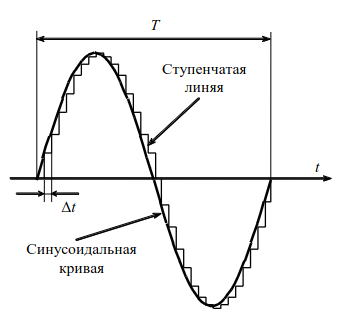
\includegraphics[width=0.4\textwidth]{../image/apr.png}
    \caption{Ступенчатая аппроксимация.}
	\end{figure}
	
\subsection{CORDIC}
	Следующий метод тоже предполагает вычисление отсчётов. Для генерации сигналов также применяется итерационный метод CORDIC. 
	%<<CORDIC --- это аббревиатура от Coordinate Rotation Digital Computer: цифровое вычисление поворота системы координат. Алгоритм "цифра за цифрой" был разработан для аппаратного поворота вектора на плоскости с помощью простых операций "сдвиг регистра вправо" и сложение/вычитание регистров.>>~\cite{cordic}. 
	Аббревиатура расшифровывается как Coordinate Rotation Digital Computer, что означает цифровое вычисление поворота системы координат. Ещё этот алгоритм называют <<цифра за цифрой>>. Он был разработан для аппаратного поворота вектора на плоскости. Для этого использовались простые операции сдвиг вправо и сложение или вычитание регистров~\cite{dds_en}.
	Смысл итерационного метода заключается в том, чтобы построить следующую последовательность: $y_{i+1}=f(y_{i})$, сходящейся к функции $y(x)$. Математической моделью в данном методе является единичная окружность с парой векторов, исходящих из центра~\cite{cordic}.
	
	\begin{figure}[H]
    \centering
    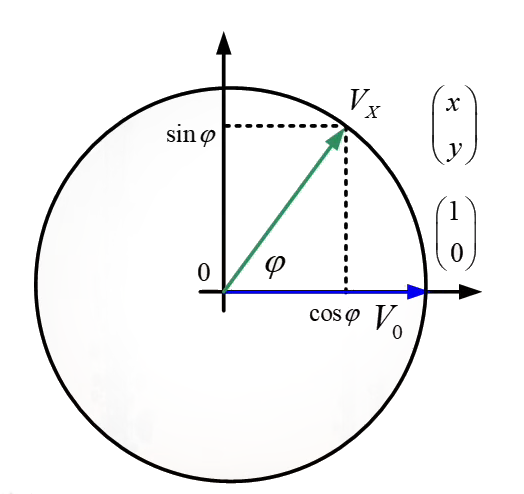
\includegraphics[width=0.4\textwidth]{../image/cordic.png}
    \caption{Математическая модель CORDIC.}
	\end{figure}

	Вектор $V_{x}$ отклонён от горизонтальной оси на угол являющимся аргументов функции. Второй вектор $V_{0}$ будет производить вращение от начальной точки относительно начала координат. Координаты векторов имеют значения $sin$ и $cos$ угла, на который вектор отклоняется от горизонтальной оси. 

	Для вектора $V_{0}$: $cos\;0 = 1$, $sin\;0 = 0$. 

	Для вектора $V_{x}$: $cos\;\phi = x$, $sin\;\phi = y$.

	Необходимо найти координаты вектора $V_{x}$ $x$ и $y$ после поворота на угол $\phi$. Координаты вычисляются по тригонометрическим формулам:
	\begin{gather}
	x=x_{0}*cos\;\phi-y_{0}*sin\;\phi, \\
	y=x_{0}*sin\;\phi+y_{0}*cos\;\phi. 
	\end{gather}
	
	Так как $tan\;\phi=\dfrac{sin\;\phi}{cos\;\phi}$, то можно выразить $sin\;\phi=tan\;\phi*cos\;\phi$ и выполнить преобразование формул. Тогда получим:
	\begin{gather}
	x=cos\;\phi(x_{0}-y_{0}*tan\;\phi), \\
	y=cos\;\phi(y_{0}+x_{0}*tan\;\phi). 
	\end{gather}
	
	\begin{figure}[H]
    \centering
    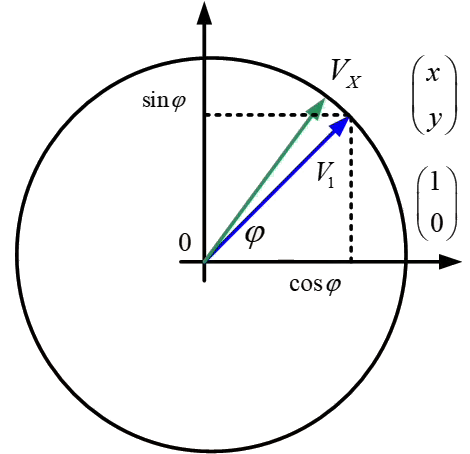
\includegraphics[width=0.4\textwidth]{../image/cordic2.png}
    \caption{Поворот вектора.}
	\end{figure}

	Если задавать такой угол поворота, что $tan\;\phi = \pm 2^{-i}$, где $i$ --- целое число, то умножение $x_{0}$ и $y_{0}$ сведётся к простому сдвигу их значений вправо на $i$ разрядов, так как деление на 2 представляет из себя побитовый сдвиг числа право.

	Произвольный угол можно представить в виде суммы углов:
	\begin{gather}
	\phi_{i}=\pm atan2^{-i}, 
	\end{gather}	
	где $i = 0, 1, 2,$ и т.д.

	Тогда операция поворота вектора будет состоять из последовательных простых поворотов. В каждой итерации проводятся следующие вычисления:
	\begin{enumerate}
	\item Направление поворота (1.10).
	\item Значение координаты $x$ (1.11).
	\item Значение координаты $y$ (1.12).
	\item Отклонение вектора	(1.13).
	\end{enumerate}
	\begin{gather}
	\sigma_{i} 	= sign(z_{i}) \\
	x_{i+1} = x_{i} - \sigma_{i}*y_{i}*2^{-i} \\
	y_{i+1} = y_{i} + \sigma_{i}*x_{i}*2^{-i} \\
	z_{i+1} = z_{i} - \sigma_{i}*atan(z^{-i}) 
	\end{gather}
	
	Данный алгоритм применим для генерации синуса и его применение целесообразно только при необходимости быстродействия и высокой точности системы.
	
\subsection{Табличный метод}		
	В табличном методе генерации сигналов предполагается, что заранее вычисленные отсчёты хранятся в памяти. То есть никаких вычислений не требуется и генерация сводится к тому, что в порт цифро-аналогового преобразователя нужно вывести ячейку по заданному адресу. 
	%<<Достоинством этого метода является меньшее время, затрачиваемое на формирование отсчета и, как следствие, возможность генерации сигналов с более высокой частотой. Недостатком является необходимость иметь большой объем памяти данных.>>~\cite{leso}. 
	Плюсом метода является то, что ему нужно меньше времени, чтобы сформировать отсчёт, т.к. он уже посчитан, следовательно, можно добиться более высокой частоты сигнала. Минусом же является необходимость хранения отсчётов, что может затратить объём памяти~\cite{leso}.
	
	Частота сигнала будет зависеть от опорной частоты устройства.
	\begin{gather}
	f_{out}=\dfrac{f_{clk}}{n}
	\end{gather}	
	
	где n --- количество отсчётов (длина таблицы).	
	
	\begin{figure}[H]
	\centering
    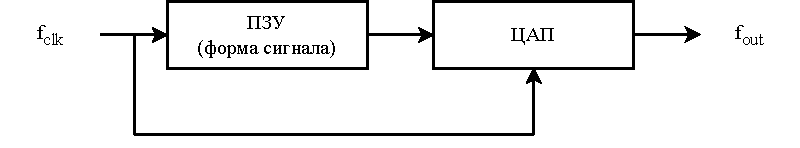
\includegraphics[width=0.9\textwidth]{../image/table_func.pdf}
    \caption{Функциональная схема табличного метода.}
	\end{figure}
	
	Управлять частотой устройства не всегда удобно. При желании уменьшить частоту сигнала придётся добавлять какую-то задержку в цикл, а что делать, если появилась необходимость увеличить частоту и код уже максимально оптимизирован. К примеру максимальная частота, которой удалось достигнуть 10 кГц и на большее наше устройство уже не способно. Так как увеличить частоту опроса таблицы уже невозможно, то нужно уменьшить её длину. То есть чтобы нам получить на выходе 20 кГц мы должны будем выводить каждый второй отсчёт таблицы, если 30 кГц, то каждый третий и т. д. Это хороший вариант, но тогда возникает проблема как дополнить программу, чтобы она пропускала нужное количество отсчётов.



\subsection{Метод DDS}	

	К табличным методам относится также метод прямого цифрового синтеза или как его ещё называют метод DDS и он решает проблему, в которую упирается обычный табличный метод. %<<Прямой цифровой синтез (от англ. DDS – Direct Digital Synthesizer) – метод, позволяющий получить аналоговый сигнал (обычно это синусоидальный сигнал, пилообразный, последовательность треугольных импульсов) за счет генерации временной последовательности цифровых отсчетов и их дальнейшего преобразования в аналоговую форму посредством ЦАП.>>~\cite{leso}. 
	DDS (Direct Digital Synthesizer) или прямой цифровой синтез, в переводе с английского, представляет собой метод, который позволяет создавать аналоговые сигналы путем генерации цифровой последовательности отсчётов и последующего преобразования этих отсчетов из цифрового вида в аналоговый с помощью ЦАП~\cite{leso}.
	
	На рисунке 1.14 изображена структурная схема DDS с аккумулятором фазы.
	
	Частота сигнала в этой архитектуре определяется следующей формулой:
	\begin{gather}
	f_{out}=\dfrac{D * f_{clk}}{2^{A}},
	\end{gather}
		
	где $f_{out}$ --- выходная частота, 
	
	$f_{clk}$ --- частота устройства, 
	
	$D$ --- код частоты, 
	
	$A$ --- разрядность аккумулятора фазы.
	
	Благодаря разрядности аккумулятора фазы можно определять насколько точно будет регулироваться частота выходного сигнала.
	
	\begin{figure}[H]
    \centering
    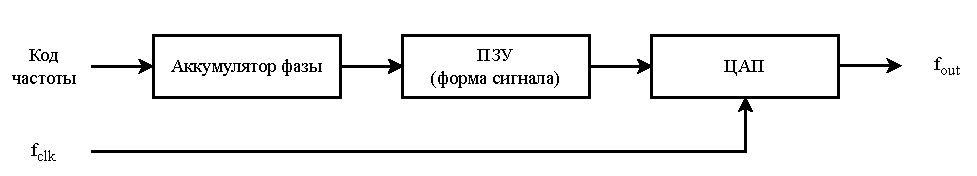
\includegraphics[width=0.9\textwidth]{../image/dds_func.pdf}
    \caption{Структурная схема DDS с аккумулятором фазы.}
	\end{figure}
	
	В аккумуляторе фазы и есть ключевое отличие метода DDS от простого табличного синтеза. Аккумулятор фазы представляет из себя регистр, в котором в каждом такте работы устройства происходит перезагрузка величины и прибавляется заданный код частоты. Приращение зависит как раз-таки от кода частоты и регулирует это значение. Таким образом, происходит вычисление какой отсчёт нужно отправить в порт цифро-аналогового преобразователя. Ещё одним отличием от табличного способа генерации является работа на фиксированной частоте. Алгоритм метода DDS можно описать блок-схемой на рисунке 1.14.
	
	\begin{figure}[H]
    \centering
    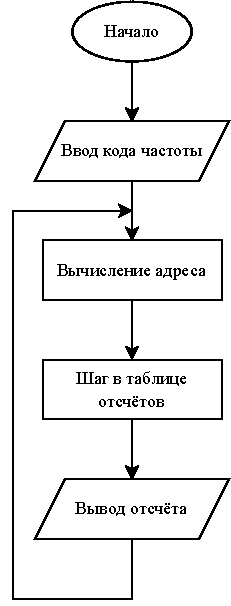
\includegraphics[width=0.35\textwidth]{../image/dds_block.pdf}
    \caption{Алгоритм метода DDS.}
	\end{figure}
	
	С помощью данного метода можно производить синтез не только стандартных форм сигналов, но и создавать произвольные формы. Метод DDS позволяет управлять цифровым способом амплитудой и фазой сигнала, а также лежит во основе многих приборов~\cite{dds_en}.
	
\section{Вывод из первой главы}
	Таким образом, можно сделать вывод о том, что среди генераторов сигналов наиболее  выделяются функциональные генераторы своей универсальностью и гибкостью. Они способны создавать различные функциональные зависимости, что позволяет генерировать сигналы разной формы, включая синусоидальные, треугольные и прямоугольные сигналы в широком спектре частот. Это делает их очень полезными для тестирования, исследования и отладки электронной аппаратуры. В следствие этого было принято решение разрабатывать функциональный генератор сигналов. В качестве метода генерации сигнала был выбран метод DDS за его простоту реализации и гибкость.
	
	